\documentclass[12pt,letter]{article}
\usepackage{geometry}\geometry{top=0.75in}
\usepackage{amsmath}
\usepackage{amssymb}
\usepackage{mathtools}
\usepackage{xcolor}	% Color words
%\usepackage{cancel}	% Crossing parts of equations out
\usepackage{tikz}    	% Drawing 
\usetikzlibrary{positioning} % prevent stuff from overlapping
\usetikzlibrary{calc}   % 
\usepackage{pgfplots}   % Other plotting
\usepgfplotslibrary{colormaps,fillbetween}
\usepackage{placeins}   % Float barrier
\usepackage{hyperref}   % Links
\usepackage{tikz-qtree} % Trees
\usepackage{graphicx}
\usepackage{subcaption}
\usepackage{multicol}
\usepackage{listings}

\tikzset{
    ->, 
    level distance = 12em,
    minimum size=2em,
    %edge from parent/.style={draw,thick},
    level 1/.style={sibling distance=6em},
    level 2/.style={sibling distance=3em},
    thick/.style = {line width=1.5pt},
    extra thick/.style = {line width=3.5pt},
    red node/.style={shape=circle,draw=red,fill=red!40,thick,inner sep=1.2},
    blue node/.style={shape=circle,draw=blue,fill=blue!40,thick,inner sep=1.2}
}

% Don't indent
\setlength{\parindent}{0pt}
% Function to replace \section with a problem name specifically formatted
\newcommand{\problem}[1]{\vspace{3mm}\Large\textbf{{Problem {#1}\vspace{3mm}}}\normalsize\\}
% Formatting function, like \problem
\newcommand{\ppart}[1]{\vspace{2mm}\large\textbf{\\Part {#1})\vspace{2mm}}\normalsize\\}
\newcommand{\documentation}[1]{\vspace{2mm}\large\textbf{\\Documentation{#1}\vspace{2mm}}\normalsize\\}
% Formatting 
\newcommand{\condition}[1]{\vspace{1mm}\textbf{{#1}:}\normalsize\\}

\begin{document}
\title{CIS 510 Assignment 2}
\author{Steven Walton}
\maketitle
\problem{P1}
Program expects an input where the first line is the number of players
and each subsequent line is the grand coalition of a subset of players surrounded
by curly braces and comma separated with the value of that coalition.
An example input file is shown here
\begin{figure}[h]
    \centering
\begin{lstlisting}
4
{1},30
{2},40
{3},25
{4},45
{1,2},50
{1,3},60
{1,4},80
{2,3},55
{2,4},70
{3,4},80
{1,2,3},90
{1,2,4},120
{1,3,4},100
{2,3,4},115
{1,2,3,4},140
\end{lstlisting}
\end{figure}

The program can be run with the following options. Not that only the input file
is required, but it is suggested to specify the output file. 
\begin{figure}[h!]
    \centering
\begin{lstlisting}
python coalition.py --help
usage: coalition.py -i <input file> -o <output file>
-h, --help       prints this message
-i, --input      sets the input file
-o, --output     sets the output file: defaults to optimalCS.txt
\end{lstlisting}
\end{figure}
\FloatBarrier

\problem{Q1}
Consider the ``cross-out" game. In this game one writes down "1,2,3". Player
1 can cross out a single number or any 2 adjacent number (12,23). Player
2 then gets to make the same type of action. The winner is the one who crosses
out the last number.

\ppart{Q1.1}
We'll create a tree where the text within the nodes denote what available choices
to the current player and where the edges show what numbers the player picked.

\begin{figure}[h]
\centering
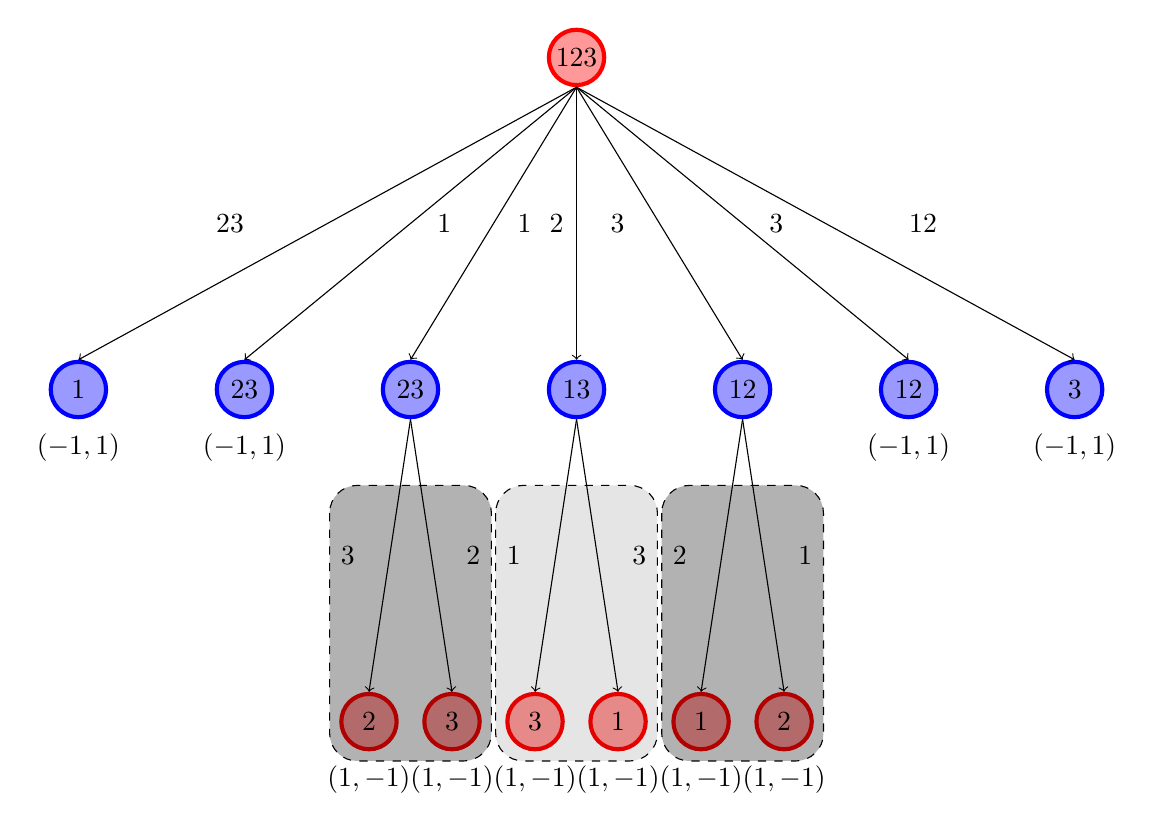
\begin{tikzpicture}
    \node(0)[red node]{123}
        child { node(23) [blue node,label=below:{$(-1,1)$}] {1} edge from parent node [left,xshift=-25]{$23$} }
        child { node(1-23) [blue node, label=below:{$(-1,1)$}] {23} edge from parent node [right,xshift=2]{$1$} }
        child { node(1) [blue node] {23} 
            child { node(1-3) [red node,label=below:{$(1,-1)$}] {2} edge from parent node [left,xshift=-5]{$3$} }
            child { node(1-2) [red node,label=below:{$(1,-1)$}] {3} edge from parent node [right,xshift=5]{$2$} }
            edge from parent node[right,xshift=1]{$1$}}
        child { node(2) [blue node] {13}
            child { node(2-1) [red node,label=below:{$(1,-1)$}] {3} edge from parent node [left,xshift=-5]{$1$} }
            child { node(2-3) [red node,label=below:{$(1,-1)$}] {1} edge from parent node [right,xshift=5]{$3$} }
            edge from parent node[left,xshift=3]{$2$}}
        child { node(3) [blue node] {12} 
            child{ node(3-2) [red node,label=below:{$(1,-1)$}] {1} edge from parent node [left,xshift=-5] {$2$} }
            child{ node(3-1) [red node,label=below:{$(1,-1)$}] {2} edge from parent node [right,xshift=5] {$1$} }
            edge from parent node[left, xshift=-5]{$3$} }
        child { node(3-12) [blue node,label=below:{$(-1,1)$}] {12} edge from parent node [right,xshift=2]{$3$} }
        child { node(12) [blue node,label=below:{$(-1,1)$}] {3} edge from parent node [right,xshift=25] {$12$} }
            ;
    \draw[anchor=text,dashed,rounded corners=10,fill=black,fill opacity=0.3]($(1-3) + (-0.5,3)$)rectangle($(1-2) + (0.5,-0.5)$);
    \draw[anchor=text,dashed,rounded corners=10,fill=black,fill opacity=0.1]($(2-1) + (-0.5,3)$)rectangle($(2-3) + (0.5,-0.5)$);
    \draw[anchor=text,dashed,rounded corners=10,fill=black,fill opacity=0.3]($(3-2) + (-0.5,3)$)rectangle($(3-1) + (0.5,-0.5)$);
\end{tikzpicture}
    \caption{Nim game: Pick a maximum of 2 adjacent numbers}
    \label{fig:nim}
\end{figure}
Looking at Figure \ref{fig:nim} we can see that the boxed subgames player 1
can always win if player 2 picks a single number. The darker boxes denote where
player 2 can win by crossing out adjacent numbers (this is equivalent to choosing
the blue nodes adjacent to these boxes and player 2 finishing the game).

This leaves two sub perfect games where player 1 always wins. Player one picks
either \{2,3\} or \{2,1\} and player 2 can choose either \{1\} or \{3\} (respective
to player 1's plays). Player 1 dominates this game because they can force player
2 into a losing action.
\begin{figure}[h]
\centering
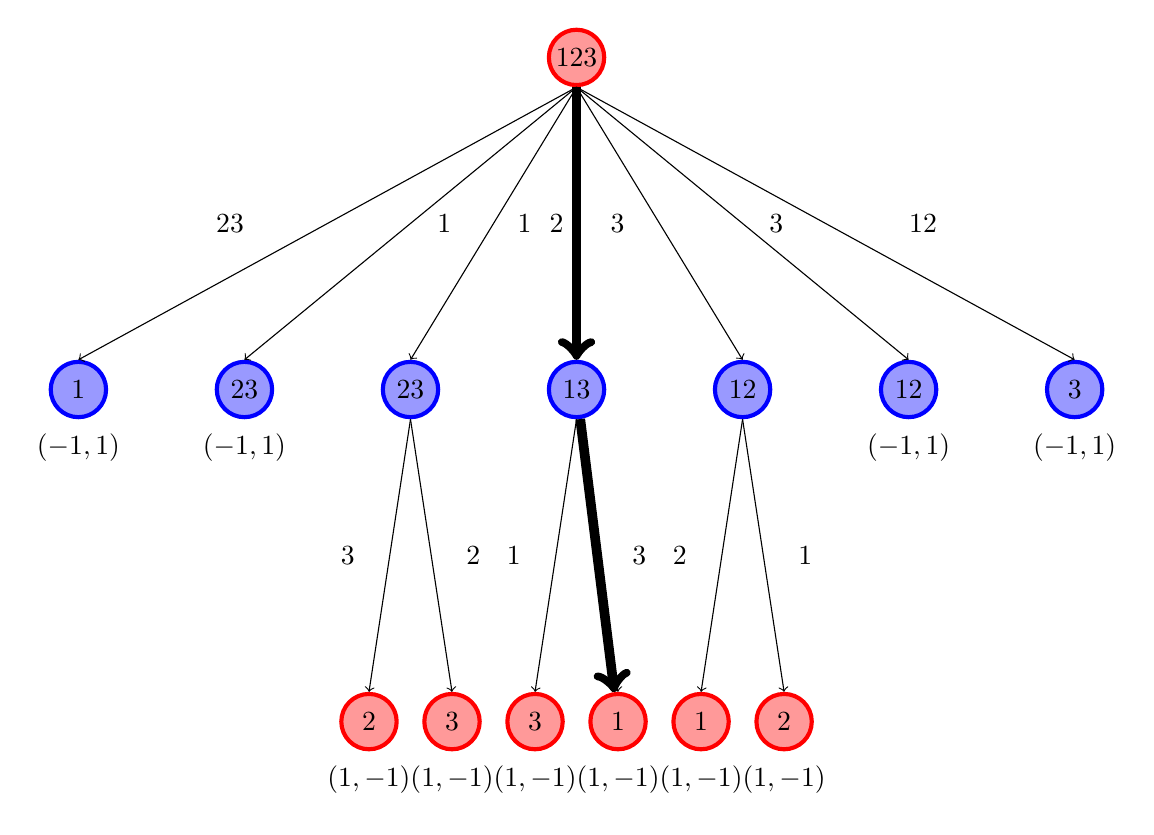
\begin{tikzpicture}
    \node(0)[red node]{123}
        child { node(23) [blue node,label=below:{$(-1,1)$}] {1} edge from parent node [left,xshift=-25]{$23$} }
        child { node(1-23) [blue node, label=below:{$(-1,1)$}] {23} edge from parent node [right,xshift=2]{$1$} }
        child { node(1) [blue node] {23} 
            child { node(1-3) [red node,label=below:{$(1,-1)$}] {2} edge from parent node [left,xshift=-5]{$3$} }
            child { node(1-2) [red node,label=below:{$(1,-1)$}] {3} edge from parent node [right,xshift=5]{$2$} }
            edge from parent node[right,xshift=1]{$1$}}
        child { node(2) [blue node] {13}
            child { node(2-1) [red node,label=below:{$(1,-1)$}] {3} edge from parent node [left,xshift=-5]{$1$} }
            child { node(2-3) [red node,label=below:{$(1,-1)$}] {1} edge from parent node [right,xshift=5]{$3$} }
            edge from parent node[left,xshift=3]{$2$}}
        child { node(3) [blue node] {12} 
            child{ node(3-2) [red node,label=below:{$(1,-1)$}] {1} edge from parent node [left,xshift=-5] {$2$} }
            child{ node(3-1) [red node,label=below:{$(1,-1)$}] {2} edge from parent node [right,xshift=5] {$1$} }
            edge from parent node[left, xshift=-5]{$3$} }
        child { node(3-12) [blue node,label=below:{$(-1,1)$}] {12} edge from parent node [right,xshift=2]{$3$} }
        child { node(12) [blue node,label=below:{$(-1,1)$}] {3} edge from parent node [right,xshift=25] {$12$} }
            ;
    \draw[extra thick, fill=black](0)--(2);
    \draw[extra thick, fill=black](2)--(2-3);
\end{tikzpicture}
    \caption{Nim game: Subgame Perfect Nash Equilibrium 2-3-1} 
\end{figure}
\begin{figure}[h]
\centering
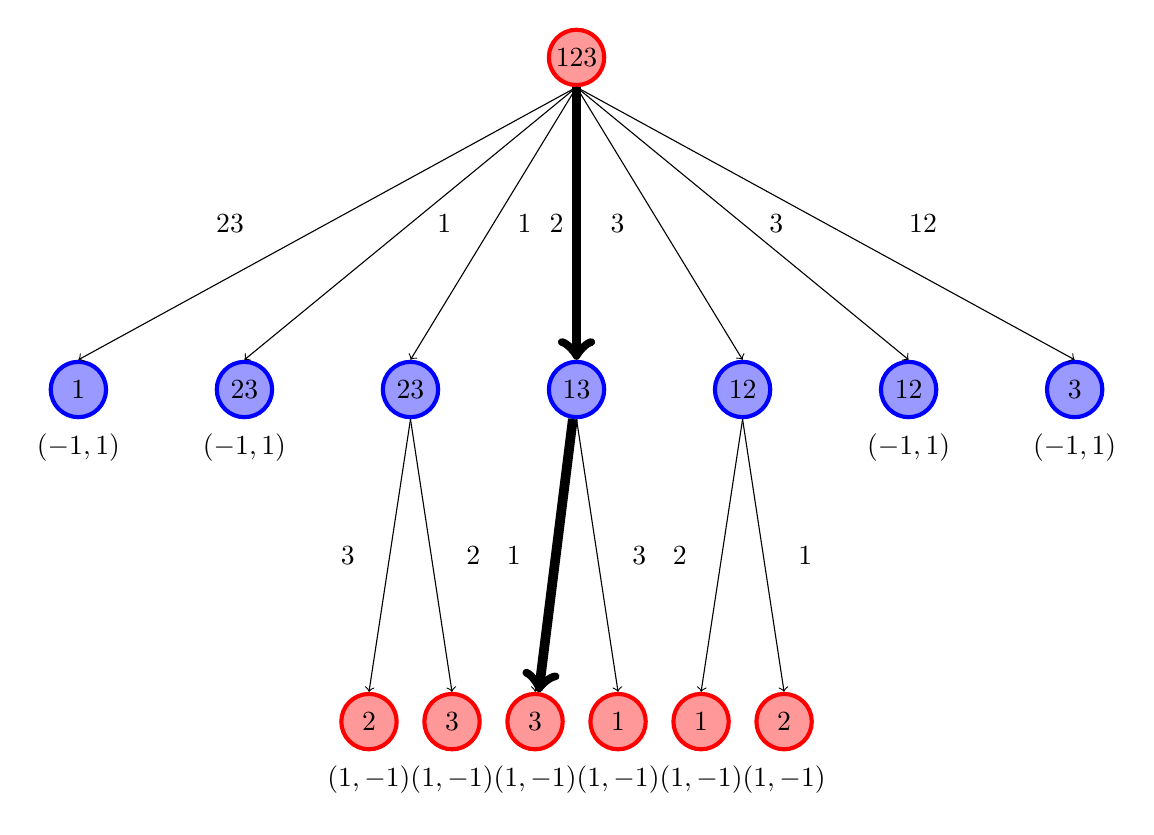
\begin{tikzpicture}
    \node(0)[red node]{123}
        child { node(23) [blue node,label=below:{$(-1,1)$}] {1} edge from parent node [left,xshift=-25]{$23$} }
        child { node(1-23) [blue node, label=below:{$(-1,1)$}] {23} edge from parent node [right,xshift=2]{$1$} }
        child { node(1) [blue node] {23} 
            child { node(1-3) [red node,label=below:{$(1,-1)$}] {2} edge from parent node [left,xshift=-5]{$3$} }
            child { node(1-2) [red node,label=below:{$(1,-1)$}] {3} edge from parent node [right,xshift=5]{$2$} }
            edge from parent node[right,xshift=1]{$1$}}
        child { node(2) [blue node] {13}
            child { node(2-1) [red node,label=below:{$(1,-1)$}] {3} edge from parent node [left,xshift=-5]{$1$} }
            child { node(2-3) [red node,label=below:{$(1,-1)$}] {1} edge from parent node [right,xshift=5]{$3$} }
            edge from parent node[left,xshift=3]{$2$}}
        child { node(3) [blue node] {12} 
            child{ node(3-2) [red node,label=below:{$(1,-1)$}] {1} edge from parent node [left,xshift=-5] {$2$} }
            child{ node(3-1) [red node,label=below:{$(1,-1)$}] {2} edge from parent node [right,xshift=5] {$1$} }
            edge from parent node[left, xshift=-5]{$3$} }
        child { node(3-12) [blue node,label=below:{$(-1,1)$}] {12} edge from parent node [right,xshift=2]{$3$} }
        child { node(12) [blue node,label=below:{$(-1,1)$}] {3} edge from parent node [right,xshift=25] {$12$} }
            ;
    \draw[extra thick, fill=black](0)--(2);
    \draw[extra thick, fill=black](2)--(2-1);
\end{tikzpicture}
    \caption{Nim game: Subgame Perfect Nash Equilibrium 2-1-3}
\end{figure}

\FloatBarrier
\ppart{Q1.2}
This is a solved game where player 1 can always win.

First let's consider the game where a player could only cross out a single number.

This game is also solved! If it is an odd sized game then player 1 can 
always win, otherwise player 2 can always win. This is because if the size 
is odd then player 1 can place a binary partition and split the game into any 
two sub games (like how in Figure ~\ref{fig:nim} Player 1 splits the game into 
two odd sized games by picking 2). Player 2 will then be the first player on one sub game 
and player 1 will be the second player in the second sub game (assuming players
play optimally, this is easy to see). If the second 
player wins any even game, then we can see that player 1 will always win this 
sub game (because it is even and they are the second player for an even 
sized game). 

This tells us how to win many different variations of this game! The key is to 
be a specific player and control if the game is even or odd. By being able to
pick up to two numbers, Player 1 can always make this control. 

As an example, let's assume that Player 1 wants to keep a subgame odd. If Player
2 picks 1 then Player 1 picks 2 (because $1+2=3$ which is odd). If Player 2 picks
2, then Player 1 picks 1 (because $2+1=3$ which is odd). Similarly, Player 1
can keep a subgame even. 

Knowing this, all Player 1 needs to do is keep track of the subgames and which
ones they need to win or lose (all that matters is that they win the last one).


\problem{2}
\begin{table}
    \centering
\begin{tabular}{|c|c|c|c|c|c|c|}
    \hline
       & L & R     & Ll& Lr    & LlU & LlD\\
    \hline
    A  & 0 & (1,1) & 0 & (2,3) & 0 & 0\\
    \hline
    B  & 0 & (1,1) & 0 & (3,2) & 0 & 0\\
    \hline
    AC & 0 & (1,1) & 0 & (2,3) & (4,1) & (1,4)\\
    \hline
    AD & 0 & (1,1) & (3,4) & (2,3) & (3,4) & (3,4)\\
    \hline
    BE & 0 & (1,1) & (2,5) & (3,2) & (2,5) &(2,5) \\
    \hline
    BF & 0 & (1,1) & 0 & (3,2) & (2,3) & (3,2)\\
    \hline
\end{tabular}
    \label{tab:EFG}
    \caption{Payoff Structure of Game}
\end{table}

\ppart{Q2.1}
Realization Plan Player 1
\begin{align*}
    r_1(\oslash) &= r_1(L) + r_1(R) = 1 \\
    r_1(L) &= r_1(Ll) + r_1(Lr) = 0.6\\
    r_1(R) &= r_1(Rl) + r_1(Rl) = 0.4\\
    r_1(Ll) &= r_1(LlU) + r_1(LlD) = 0.4\\
    r_1(Lr) &= r_1(LrU) + r_1(LrD) = 0.2\\
    r_1(LlU) &= 0.2\\
    r_1(LlD) &= 0.2\\
    r_1(LrU) &= 0.1\\
    r_1(LrD) &= 0.1\\
    r_1(\oslash),r_1(L),r_1(R),&r_1(Ll),r_1(Lr),r_1(LlU), r_1(LlD), r_1(LrU), r_1(LrD) \geq 0\\
\end{align*}


Realization Plan Player 2
\begin{align*}
    r_2(\oslash) &= r_2(A) + r_2(B) = 1\\
    r_2(A) &= r_2(AC) + r_2(AD) = 0.5\\
    r_2(B) &= r_2(BC) + r_2(BD) = 0.5\\
    r_2(AC) &= 0\\
    r_2(AD) &= 0.5\\
    r_2(BE) &= 0.5\\
    r_2(BF) &= 0\\
    r_2(\oslash),r_2(A),r_2(B),&r_2(AC),r_2(AD),r_2(BE),r_2(BF) \geq 0
\end{align*}
Strategies $AC$ and $BF$ are set to 0 because under those circumstances it would
never be a good idea for Player 2 to take those actions. 

\ppart{Q2.2}
We have

Player 1:
\begin{align*}
    &\beta_1(L) = r_1(L) = \frac35
    &\beta_1(R) = r_(R) = \frac25\\
    &\beta_1(l) = \frac{r_1(Ll)}{r_1(L)} =\frac23
    &\beta_1(r) = \frac{r_1(Lr)}{r_1(L)} =\frac13\\
    &\beta_1(U) = \frac{r_1(LlU)}{r_1(Ll)} = \frac12
    &\beta_1(D) = \frac{r_1(LlD)}{r_1(Ll)} = \frac12
\end{align*}

%We have a possible behavioral strategy: P1(L:0.6,R:0.4),(l:0.3,r:0.7),(U:0.8,D:0.2)

Player 2:
\begin{align*}
    &\beta_2(A) = r_2(A) = \frac12
    &\beta_2(B) = r_2(B) = \frac12\\
    &\beta_2(C) = \frac{r_2(AC)}{r_2(A)} = 0 
    &\beta_2(D) = \frac{r_2(AD)}{r_2(A)} = 1\\
    &\beta_2(E) = \frac{r_2(BE)}{r_2(B)} = 1
    &\beta_2(F) = \frac{r_2(BF)}{r_2(B)} = 0
\end{align*}
%We have a possible behavioral strategy: P2(A:0.5,B:0.5),((C:0,D:1.),(E:1.,F:0.))

\ppart{Q2.3}
\begin{align*}
    \max &\sum\limits_{\sigma_2\in\Sigma_2}\left(\sum\limits_{\sigma_1\in\Sigma_1}g_2(\sigma_1,\sigma_2)r_1(\sigma_2)\right)r_2(\sigma_2)\\
    s.t \hspace{1em}& r_2(\oslash) = 1\\
        & \sum\limits_{\sigma_2'\in Ext_2(I)}r_2(\sigma_2') = r_2(seq_2(I))\\
        & r_2(\sigma_2)\geq 0
\end{align*}
Where $g_2(\sigma_1,\sigma_2)$ are the combinations or realization plans from
player 1 and 2, where $\sigma_1\in\Sigma_1$ and $\sigma_2\in\Sigma_2$
\begin{table}[h]
    \centering
    \begin{tabular}{c|c}
        \hline
        $\Sigma_1$ & $\Sigma_2$\\
        \hline
        $\oslash$ & $\oslash$ \\
        L & A\\
        R & B\\
        Ll & AC\\
        Lr & AD\\
        LlU & BE\\
        LlD & BF\\
    \end{tabular}
\end{table}

As a mathematician I thought we were done here, because this is a compact 
representation of all the information needed to solve the problem and this could
could programmatically be done.

We know that $g_2$ and $r_1$ are constants and that $r_2$ is the only variable.
We can do some careful reduction to make the expansion easier. We note that
all $g(*,\oslash)=0$ Similarly any plan that does not reach a leaf node results
in $0$. We use $*$ similar to a wild character. 
\begin{align*}
    &\max \sum\limits_{\sigma_2\in\Sigma_2}r_2(\sigma_2)\left(\sum\limits_{\sigma_1\in\Sigma_1}g_2(\sigma_1,\sigma_2)r_1(\sigma_1)\right)\\
    &=\max r_2(\oslash)(0)\\
    &+r_2(A)[g(R,A)r_1(R) + g(Lr,A)r_1(Lr)]\\
    &+r_2(AD)[g(R,AD)r_1(R) + g(Lr,AD)r_1(Lr) + g(Ll,AD)r_1(Ll)]\\
    &+r_2(B)[g(R,B)r_1(R) + g(Lr,B)r_1(Lr)]\\
    &+r_2(BE)[g(R,BE)r_1(R) + g(Lr,BE)r_1(Lr) + g(Ll,BE)r_1(Ll)]\\
    &=\max r_2(A)[(1)(0.4) + (3)(0.2)] + r_2(AD)[(1)(0.4) + (3)(0.2) + (4)(0.2)]\\
    &+r_2(B)[(1)(0.4) + (2)(0.4)] + r_2(BE)[(1)(0.4) + (2)(0.2) + (5)(0.4)]\\
    &=\max \left(r_2(A) + r_2(AD)(1.8) + r_2(B)(1.2) + r_2(BE)(2.8)\right)
\end{align*}



\end{document}
